\documentclass[tikz,border=2pt]{standalone}
\usepackage{amsmath}
\begin{document}
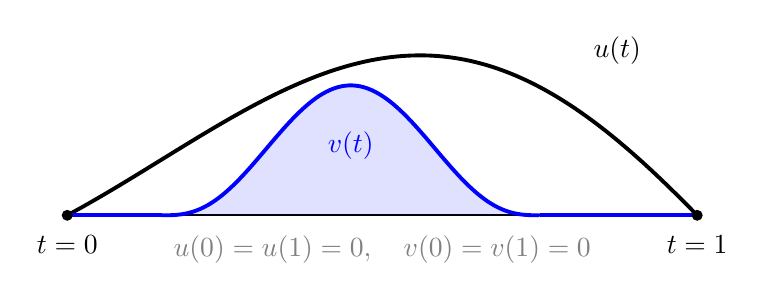
\begin{tikzpicture}[xscale=8, yscale=2.2]
    % domain [0,1]
    \draw[thick] (0,0) -- (1,0);
    % true solution u (asymmetric, vanishes at 0 and 1)
    \draw[line width=1.4pt, black, domain=0:1, samples=120, smooth]
        plot (\x, {sin(180*\x)*(1 + 0.9*\x)/1.6});
    % test function v: smooth bump, vanishes at 0 and 1
    \fill[blue, opacity=0.12, domain=0.15:0.75, samples=100, smooth]
        (0.15,0) -- plot (\x, {0.75*(1 - ((\x-0.45)/0.3)^2)^3}) -- (0.75,0) -- cycle;
    \draw[line width=1.4pt, blue, domain=0.15:0.75, samples=100, smooth]
        plot (\x, {0.75*(1 - ((\x-0.45)/0.3)^2)^3});
    \draw[line width=1.4pt, blue] (0,0) -- (0.15,0);
    \draw[line width=1.4pt, blue] (0.75,0) -- (1,0);
    % labels
    \node[black, right] at (0.82,0.95) {$u(t)$};
    \node[blue] at (0.45,0.4) {$v(t)$};
    % boundary points
    \fill[black] (0,0) circle (0.25pt and 0.9pt);
    \fill[black] (1,0) circle (0.25pt and 0.9pt);
    \node[below=4pt] at (0,0) {$t = 0$};
    \node[below=4pt] at (1,0) {$t = 1$};
    \node[below=4pt, gray] at (0.5,0) {$u(0) = u(1) = 0, \quad v(0) = v(1) = 0$};
\end{tikzpicture}
\end{document}
